%%=============================================================================
%% Methodologie
%%=============================================================================

\chapter{\IfLanguageName{dutch}{Methodologie}{Methodology}}
\label{ch:methodologie}

%% TODO: Hoe ben je te werk gegaan? Verdeel je onderzoek in grote fasen, en
%% licht in elke fase toe welke stappen je gevolgd hebt. Verantwoord waarom je
%% op deze manier te werk gegaan bent. Je moet kunnen aantonen dat je de best
%% mogelijke manier toegepast hebt om een antwoord te vinden op de
%% onderzoeksvraag.
\section{\IfLanguageName{dutch}{Inleiding}{Preface}}
\label{sec:methodologie-inleiding}

In dit hoofdstuk worden de belangrijkste keuzes besproken en de verbonden technische aspecten. Zoals in de probleemstelling aangegeven zijn volgende 4 doelen steeds in dachte gehouden:
\begin{itemize}
    \item Foto's zoekbaar maken door middel van AI
    \item De oplossing moet gemakkelijk te gebruiken zijn
    \item De oplossing moet breed bruikbaar zijn; voor veel verschillende soorten foto-archieven
    \item Foutmarge van maximaal 15\%
\end{itemize}

\section{\IfLanguageName{dutch}{Keuze van computer vision model}{Choice of computer vision model}}
\label{sec:keuze-van-computer-vision}
Computer vision is een breed veld binnen machine learning waarbij verschillende technieken gebruikt kunnen worden om classificatie uit te voeren. Na inleidend onderzoek werd duidelijk dat er een beslissing moest gemaakt worden op 3 vlakken, iedere keuze vloeit voort uit de vorige:
\begin{enumerate}
    \item Wordt er zelf een model getraind of wordt er gebruikt gemaakt van een pre-trained model
    \item Specifieke of algemene herkenning
    \item Welke computer vision API providers worden er gebruikt
\end{enumerate}

\subsection{\IfLanguageName{dutch}{Self-trained versus pre-trained}{Self-trained versus pre-trained}}
\label{sec:Self-trained-versus-pre-trained}
Self-trained computer vision modellen worden getraind op basis van data die de gebruiker aan het model aanbiedt, op basis van deze data zal het model proberen kennis op te bouwen om voorspellingen te kunnen maken. Zoals in de stand-van-zaken werd besproken is het bij computer vision belangrijk dat de data kwalitatief van hoog niveau is en dat er miljoenen afbeeldingen zijn om het model te trainen. Er zijn open datasets beschikbaar die gebruikt kunnen worden om een start te geven aan een self-trained model, de gebruiker haalt dan een pre-gelabelde dataset binnen en gebruikt die als basis voor de training. Het grootste voordeel aan self-trained modellen is dat men een grote mate van controle heeft over de trainingsdata en dat men het model kan tot in detail kan finetunen. 

Pre-trained computer vision modellen werden getraind door een organisatie op basis van grote hoeveelheden kwalitatieve data. Een gebruiker kan met een minimum aan configuratie de modellen aanspreken en voorspellingen ophalen. Aangezien de gebruiker geen invloed heeft op configuratie of training zijn de modellen vaak een 'black box', het is onduidelijk hoe het model voorspellingen maakt. Deze modellen zijn typisch aanspreekbaar via een API maar kunnen ook lokaal uitgevoerd worden.

Voor self-trained modellen is het voorzien van kwalitatieve en kwantitatieve data een te grote initiële investering voor een gemiddeld bedrijf, er kan niet verwacht worden dat een bedrijf zelf miljoenen afbeeldingen labelt in een specifiek format. Ook als er gekozen wordt voor het gebruik van een open dataset moet er te veel configuratie en finetuning gebeuren. Voor dit onderzoek werd er bijgevolg gekozen om enkel pre-trained modellen te gebruiken. Voor een gemiddeld bedrijf is het niet belangrijk om te weten hoe de voorspelling precies gebeurt, zolang de voorspellingen accuraat zijn. Het integreren met een API's is een technische taak die door een gemiddeld bedrijf kan worden uitgevoerd.

\subsection{\IfLanguageName{dutch}{Specifieke herkenning versus algemene herkenning}{Specific recognition versus general recognition}}
\label{sec:specific-versus-general}
De meeste pre-trained modellen zijn gespecialiseerd in 1 bepaalde soort herkenning, bijvoorbeeld: emoties lezen van gezichten; herkennen van planten; gezichtsherkenning. Naast de specifieke modellen zijn er ook algemene modellen, deze proberen herkenning mogelijk te maken van een zo breed mogelijk aantal onderwerpen: zowel lezen van emoties, als plantherkenning als gezichtsherkenning als .... 

Voor deze bachelorproef ligt de focus op foto-archieven, het is de bedoeling dat ongeorganiseerde foto-datasets kunnen worden aangeboden en dat er correct labels voorspeld worden. Aangezien algemene modellen breed inzetbaar zijn wordt er voor deze optie gekozen.

\subsection{\IfLanguageName{dutch}{Keuze van externe API's}{Choice of external API's}}
\label{sec:keuze-externe-API}
Er zijn verschillende API's online beschikbaar die pre-trained computer vision aanbieden specifiek getraind voor algemene herkenning. Een voordeel bij het gebruiken van API's is dat er geen lokale processing power moet gebruikt worden, een nadeel is dat herkenning niet werkt zonder een actieve internetverbinding. Bij computer vision geldt vaak 'bigger is better', hoe groter de achterliggende dataset en hoe groter de compute power tijdens training, hoe beter het resultaat. Op basis van deze insteek en na besprekingen met computer vision developers werd er beslist om met de twee grootste spelers verder te gaan, namelijk Google Vision en AWS Rekognition. Om de vergelijking volledig te maken werd er gekozen om ook te integreren met een kleinere speler genaamd imagga.

Alle externe API's voldoen aan volgende kwaliteiten:
 \begin{itemize}
     \item Mogelijkheid tot het labelen van afbeeldingen
     \item Pre-trained, algemene herkenning
     \item Weinig tot geen configuratie nodig, gemakkelijke integratie
     \item Uitgebreide API documentatie beschikbaar
     \item Mogelijkheid tot gratis verwerkingen per maand
 \end{itemize}

\section{\IfLanguageName{dutch}{Integratie met computer vision API's}{Integrating with Computer Vision API's}}
\label{sec:integratie-met-computer-vision}
Om de integratie met de 3 API's op te zetten werd er gekozen om een proof of concept applicatie te schrijven in C\# .Net Core 3.1. Deze applicatie heeft volgende doelen:
 \begin{enumerate}
    \item Via code de API's aanspreken
    \item Afbeeldingen uit de dataset aanbieden
    \item Resultaten te ontvangen
    \item Resultaten in een CSV file (Comma-Seperated Values) opslaan
\end{enumerate}

De dataset afbeeldingen werden lokaal opgeslagen in jpg format. Voor iedere afbeelding worden er per API 3 labels opgevraagd, voor iedere label wordt er ook een zekerheidsgraad opgevraagd uitgedrukt in procent. Deze zekerheidsgraad geeft aan hoe zeker de API is van het geretourneerde label. Naast de labels en de zekerheidsgraden wordt er per request bijgehouden hoeveel milliseconden de request heeft geduurd, de calls worden via een LAN-kabel op hetzelfde netwerk uitgevoerd. Alle resultaten worden naar een CSV file weggeschreven met kolommen zoals aangeduid in Figuur~\ref{fig:columnsclassification}. De sourcecode van de applicatie is terug te vinden op GitHub \footnote{https://github.com/frederikvrHogent/bachelor-proef-code}.

\begin{figure}
    \centering
    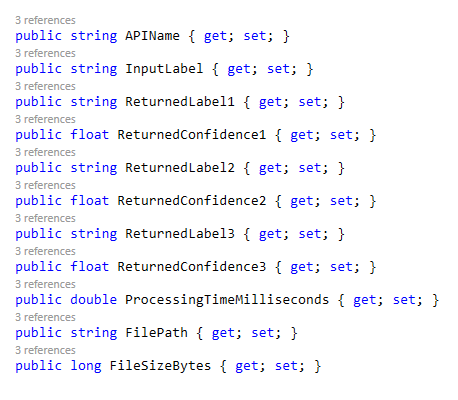
\includegraphics[width=\textwidth]{columnsclassification}
    \caption{De kolommen van de classificatie-resultaten.}
    \label{fig:columnsclassification}
\end{figure}

Volgende details van de integratie worden voor iedere provider apart besproken:
 \begin{itemize}
    \item Creatie van account
    \item Authenticatie via code
    \item Request-response flow
    \item Moeilijkheid van integratie
\end{itemize}

\subsection{\IfLanguageName{dutch}{imagga}{imagga}}
\label{sec:integration-imagga}
Opzet van een imagga account gebeurt door het invullen van persoonlijke gegevens en emailadres op de imagga website \footnote{https://imagga.com/}. Na activatie van de account kan er ingelogd worden en kan de API gebruikt worden zonder verdere configuratie. Er wordt automatisch een trial account gestart met 1000 gratis verwerkingen per maand.

Tijdens creatie van de account wordt er automatisch een API Key en een API Secret aangemaakt, deze kunnen in code gebruikt worden om een authenticatie value op te bouwen. De authenticatie value moet bij iedere request meegestuurd worden. imagga voorziet geen SDK (Software Development Kit) om de integratie met de API op te zetten maar voorziet wel uitgebreide API documentatie met code snippets in verschillende programmeertalen. Deze code snippets zijn gedetailleerd en bevatten alle nodige informatie om een request/response op te bouwen.

imagga voorziet geen functionaliteit om lokale afbeeldingen in memory te laden en deze aan de API aan te bieden, de afbeeldingen moeten eerst geupload worden naar het platform via een POST REST request. Na het uploaden wordt er via de response een 'image upload id' terug gestuurd. Deze id kan vervolgens gebruikt worden om een GET labels REST request op te bouwen, deze request laat toe om het aantal geretourneerde labels te configureren via een parameter. Zie Figuur~\ref{fig:imaggacode} voor een code snippet van de GET labels request. imagga voorziet geen SDK dus moeten alle requests en responses via code opgezet worden. Requests worden volledig via parameterisatie geconfigureerd, responses worden teruggestuurd in JSON formaat. De totale verwerkingstijd voor 1 afbeelding is de volledige tijd die nodig is om de image up te loaden en labels op te vragen, de calls worden synchroon uitgevoerd om er zeker van te zijn dat de verwerkingstijd correct wordt bijgehouden.

Opzet van een imagga acount en gebruik van de API is eenvoudig door de uitgebreide documentatie en code snippets. Omdat er geen SDK beschikbaar is moet er via code steeds een REST client worden opgebouwd en de JSON objecten moeten manueel worden gedeserialiseerd, wat voor extra code werk en complexiteit zorgt. Verder voorziet imagga geen ingebouwde functionaliteit om de API Key en API Secret buiten de code op te slaan, dit kan echter eenvoudig worden opgelost via een config file of environment variabele.

\begin{figure}
    \centering
    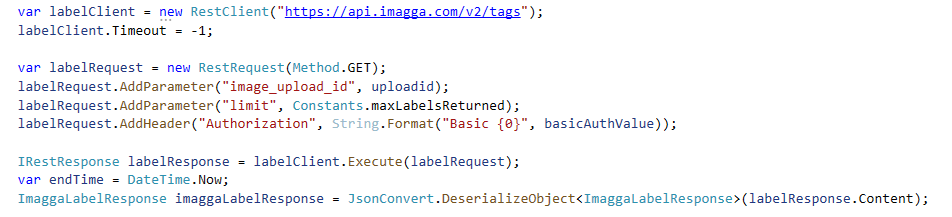
\includegraphics[width=\textwidth]{imaggacode}
    \caption{Code snippet van de GET labels call met imagga.}
    \label{fig:imaggacode}
\end{figure}

\subsection{\IfLanguageName{dutch}{AWS Rekognition}{AWS Rekognition}}
\label{sec:integration-AWS}
Een AWS account kan gecreëerd worden via de AWS website \footnote{https://portal.aws.amazon.com/billing/signup} door persoonlijke gegevens en emailadres in te vullen. Bij creatie van de account wordt automatisch de AWS Free Tier opgestart; de Free Tier is voor 12 maanden geldig en laat 5000 gratis verwerkingen per maand toe.

Vervolgens moet er een IAM user aangemaakt worden, bij gebruik van AWS services - zoals AWS Rekognition - wordt authenticatie en autorisatie steeds uitgevoerd op basis van de IAM user. Nadat de user werd aangemaakt moeten de correcte access rights worden toegewezen zodat de Rekognition API aangeroepen kan worden. Wanneer de IAM user volledig werd opgezet kan een credentials file gedownload worden vanuit de AWS console \footnote{https://console.aws.amazon.com/} die de API Key en de API Secret bevat. Deze twee keys moeten in een specifieke file format opgeslagen worden in een subfolder van de home folder genaamd ''.aws''. Naast de credentials file moet er in dezelfde folder een config file opgezet worden waarin de regio wordt gedefinieerd, voor dit onderzoek werd er voor 'eu-west' gekozen omdat deze de beste performantie heeft voor België.

Via de Visual Studio NuGet package manager kunnen de AWSSDK.Core\footnote{https://www.nuget.org/packages/AWSSDK.Core/} en AWSSDK.Rekognition\footnote{https://www.nuget.org/packages/AWSSDK.Rekognition/} packages geïnstalleerd worden. Verder zijn er C\# code snippets beschikbaar die voorbeelden geven hoe de packages gebruikt kunnen worden. De test-images kunnen in memory worden geladen en aangeboden worden aan de Rekognition client die de achterliggende AWS endpoint aanspreekt, via een input parameter wordt bepaald hoeveel labels er geretourneerd worden. De SDK verbergt de achterliggende authenticatie en REST calls wat er voor zorgt dat de calls in enkele lijnen code worden afgehandeld.

Creatie van de AWS account en IAM role kunnen verwarrend zijn voor een nieuwe gebruiker, er moeten meerdere stappen uitgevoerd worden voor er een API call kan gemaakt worden. Nadat de credentials en config correct werden opgezet is de code om de calls uit te voeren zeer eenvoudig. De AWS SDK's zorgen er voor dat de de achterliggende calls verborgen zijn en dat de consument slechts enkele lijnen code nodig heeft om de functionaliteit aan te roepen. Er zijn uitgebreide quickstarts, documentatie en codesnippets beschikbaar via de AWS console, echter zijn deze niet overzichtelijk gestructureerd.

\subsection{\IfLanguageName{dutch}{Google Vision}{Google Vision}}
\label{sec:integration-google}
Voor Google Vision gebruikt kan worden moet er een Google Cloud account worden aangemaakt, dit kan door een emailadres te registreren op de Google Cloud Console \footnote{https://console.cloud.google.com/}. Zoals bij imagga en AWS wordt er automatisch een free trial account geactiveerd. Deze free trial is geldig voor 90 dagen, en heeft 300 dollar budget voor cloud services - daarnaast worden de eerste 1000 images per maand gratis door Google Vision verwerkt.

Na opzet van de account moet er een Google Cloud project aangemaakt worden, bij het project moeten de access rights gedefinieerd worden en de Google Vision API geactiveerd worden. Na opzet van het project moet er een service account geactiveerd worden via de Google Cloud Console. De service account moet aan het project gelinkt worden en de correcte access rights krijgen, vervolgens kan er van deze service account een JSON key file gedownload worden. Deze key file bevat access keys en andere accountinformatie, het pad naar deze JSON key file wordt via een specifieke environment variabele vastgelegd. Voor de Google Vision API gebruikt kan worden moet men ook de Cloud SDK installeren, dit kan via een PowerShell command\footnote{https://cloud.google.com/sdk/docs/install}.

In Visual Studio NuGet package manager kan nu de Google Cloud Vision SDK\footnote{https://www.nuget.org/packages/Google.Cloud.Vision.V1/} geïnstalleerd worden. Er zijn C\# code snippets beschikbaar die een voorbeeld geven hoe de client gebruikt kan worden, images kunnen in memory worden geladen en rechtstreeks worden aangeboden aan de client - een inputparameter bepaalt hoeveel labels er geretourneerd worden. Zoals bij AWS verbergt de SDK de achterliggende authenticatie en REST calls, dit zorgt er voor dat de calls op enkele lijnen code kunnen worden afgehandeld, zie Figuur~\ref{fig:googlecode}.

\begin{figure}
    \centering
    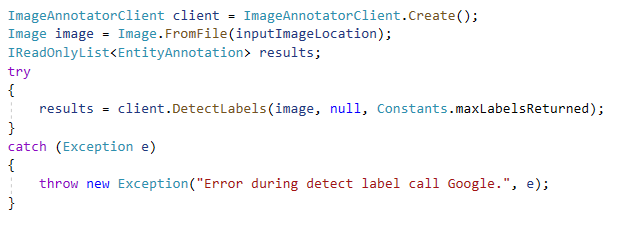
\includegraphics[width=\textwidth]{googlecode}
    \caption{Code snippet van de GET labels call met Google.}
    \label{fig:googlecode}
\end{figure}

Zoals bij AWS kan opzet en creatie van de Google Cloud account en authenticatie ingewikkeld zijn voor een nieuwe gebruiker. Echter na opzet van de credentials wordt de implementatie gemakkelijk afgewerkt, de SDK zorgt voor een eenvoudige en implementatie met de API. Ook bij Google Vision zijn er voldoende codesnippets, documentatie en quickstarts beschikbaar - de informatie is duidelijk en gestructureerd.

\section{\IfLanguageName{dutch}{Testdata}{Testdata}}
\label{sec:methodologie-data}
De dataset gebruik in dit onderzoek bestaat uit 30 gelabelde afbeeldingen afkomstig uit de Beeldbank van Archief Gent\footnote{https://beeldbank.stad.gent/} - ik draag graag mijn dank uit aan het Gents Archief om deze afbeeldingen beschikbaar te stellen en voor de aangename communicatie. Om zo nauw mogelijk aan te sluiten op de onderzoeksvraag zijn er verschillende soorten afbeeldingen gebruikt: mensen; bekende gebouwen; stadsbeelden; landschappen; interieur. Alle afbeeldingen uit deze archieven komen uit de periode 1796 tot nu. De afbeeldingen zijn een collectie van zowel foto's als postkaarten.

De afbeeldingen in de dataset zijn onder volgende categorieën verdeeld:
\begin{itemize}
    \item 15 zwart-wit foto's of postkaarten
    \item 15 foto's of postkaarten met kleur
\end{itemize}

Alle afbeeldingen in de Beeldbank werden manueel gelabeld, er is hier bij het Archief Gent momenteel geen eenduidig systeem voor. Afbeeldingen kunnen gelabeld worden door de uploader, andere worden in bulk gelabeld, bij nog andere worden er achteraf labels toegevoegd. Vooral bij de oudere zwart-wit foto's valt het op dat gedetailleerde labels ontbreken, wat een invloed zal hebben op de scoring van de labels bij het onderzoek.

Van iedere afbeelding worden de eerste 5 labels uit de Beeldbank bijgehouden in de dataset, indien er een beschrijving beschikbaar is wordt deze ook bijgehouden. Bij sommige afbeeldingen werd er in de dataset een notitie toegevoegd, deze is informatief en wordt niet gebruikt om de modellen te scoren. De URL met verwijzing naar de bron is voor iedere afbeelding beschikbaar. Wanneer er velden niet zijn ingevuld betekent het dat de data niet beschikbaar was. 

De volledige dataset kan via Google Sheets worden geraadpleegd \footnote{https://docs.google.com/spreadsheets/d/11UHeuM9SxL0aSF5OMRoSS2XG5aFBfdMBoC1CjSZI0Jg}.

\section{\IfLanguageName{dutch}{Scoren van computer vision API's}{Scoring of the Computer Vision API's}}
\label{sec:scoren-van-computer-vision}
Iedere afbeelding uit de dataset wordt aangeboden aan de 3 verschillende API's, iedere API levert 3 labels en bijhorende zekerheidsgraad af. Naast labels en de zekerheidsgraad wordt de snelheid van de API call bijgehouden. De computer vision API's zullen gescoord worden zowel op correctheid van labels als snelheid van verwerking.

\subsection{\IfLanguageName{dutch}{Scoren van de labels}{Scoring of the labels}}
\label{sec:scoren-van-labels}
Ieder label geretourneerd door een API wordt gepunt in 1 van volgende categorieën:
\begin{itemize}
    \item Volledig correct
    \item Correct
    \item Enigszins correct
    \item Niet correct
\end{itemize}

Voor iedere API wordt de hoeveelheid labels per categorie opgeteld om zo een overzicht van de algemene correctheid van de API te bekomen.

\subsubsection{\IfLanguageName{dutch}{Volledig correct}{Completely correct}}
\label{sec:completely-correct}
De label komt overeen met een label of de beschrijving uit de originele dataset voor de afbeelding in kwestie.

\subsubsection{\IfLanguageName{dutch}{Correct}{Correct}}
\label{sec:correct}
De label komt niet overeen met een label uit de originele dataset maar is wel correct voor de afbeelding in kwestie.

\subsubsection{\IfLanguageName{dutch}{Enigszins correct}{Somewhat correct}}
\label{sec:somewhat-correct}
De label komt niet overeen met een label uit de originele dataset maar is enigszins correct voor de afbeelding in kwestie. Onder deze categorie vallen labels die correct zijn voor de afbeelding maar te ruim of vaag zijn om waarde toe te voegen. Voorbeelden zijn: 'afbeelding';'foto';'vorm'.

\subsubsection{\IfLanguageName{dutch}{Niet correct}{Not correct}}
\label{sec:not-correct}
De label komt niet overeen met een label uit de originele dataset en is niet correct voor de afbeelding in kwestie. Wanneer labels een synoniem zijn van elkaar wordt er slechts 1 als correct gepunt, de andere worden als niet correct gepunt.
Bijvoorbeeld. 'bicycle'; 'bike'.


\subsubsection{\IfLanguageName{dutch}{Zekerheidsgraad thresholding}{Confidence thresholding}}
\label{sec:scoring-thresholding}
Naast de scoring van de labels wordt er ook rekening gehouden met de bijhorende zekerheidsgraad, wanneer deze API's in een productie-omgeving gebruikt worden is het belangrijk dat enkel de correcte labels behouden worden. Daarom werd er besloten dat alle labels met een zekerheidsgraad die minder is dan 75\% niet worden meegeteld voor het productie-resultaat. Er werd gekozen voor een threshold van 75\% omdat er geen zware consequenties vasthangen aan het toelaten van een incorrect label, deze threshold kan verder afgesteld worden op basis van verder onderzoek; er zou per computer vision model onderzocht kunnen worden welke threshold voor de beste resultaten zorgt.

Bij het analyseren van de resultaten wordt er per computer vision model besproken welke invloed deze threshold op het eindresultaat heeft. 

\subsection{\IfLanguageName{dutch}{Scoren van de snelheid}{Scoring of speed}}
\label{sec:scoren-of-speed}
Bij het labelen van foto-archieven is snelheid in het algemeen van minder belang, er is typisch geen tijdsdruk om de labels binnen een bepaalde tijdspanne aan te duiden. Manuele labeling duurt minstens 10 seconden of 10.000 milliseconden per foto: de persoon moet de foto openklikken; 1 of meerdere labels intypen; de labels opslaan; volgende foto selecteren. 

Het is dan ook belangrijk dat de automatische labeling via computer vision binnen dit tijdsbestek van 10 seconden blijft, op deze manier wordt ten minste de verwerkingstijd van manuele labeling geëvenaard. Snellere verwerking krijgt steeds de voorkeur op tragere verwerking.
